\documentclass[10pt]{beamer}
\usefonttheme{professionalfonts,serif}
\def\newblock{\hskip .11em plus .33em minus .07em}
\usepackage[numbers,sort]{natbib}
\renewcommand{\rmdefault}{psbx}
\usepackage[utf8]{inputenc}
\usepackage[T1]{fontenc}
\usepackage{textcomp}
\usepackage{eulervm}

\usetheme{default}           % tips from David Blei
\useinnertheme{circles}
\useoutertheme{infolines}
\setbeamertemplate{headline}{}
\setbeamertemplate{navigation symbols}{}
\setbeamerfont{itemize/enumerate subbody}{size=\normalsize}
\setbeamerfont{itemize/enumerate subsubbody}{size=\normalsize}
\usecolortheme{seahorse}
\setbeamersize{text margin left=2mm,text margin right=2mm}

\graphicspath{{../../figures/}}

\definecolor{mypine}{rgb}{0.05,0.45,0.05}
\definecolor{mycyan}{rgb}{0.0,0.9,0.9}
\newcommand{\Red}{\textcolor{red}}
\newcommand{\Blue}{\textcolor{blue}}
\newcommand{\Green}{\textcolor{mypine}}
\newcommand{\PineGreen}{\textcolor{mypine}}
\newcommand{\Magenta}{\textcolor{magenta}}
\newcommand{\Cyan}{\textcolor{mycyan}}

\newcommand{\N}{\mathcal{N}}
\newcommand{\R}{\mathbb{R}}
\newcommand{\T}{{\scriptsize^{\top}}}
\newcommand{\D}{\mathcal{D}}
\newcommand{\F}{\mathcal{F}}
\newcommand{\E}{\mathbb{E}}
\newcommand{\V}{\mathbb{V}}
\newcommand{\M}{\mathcal{M}}
\newcommand{\KL}{\mathcal{KL}}
\newcommand{\cut}[1]{}
\newcommand{\trace}{\operatorname{trace}}

\newcommand{\bmu}{{\boldsymbol{\mu}}}
\newcommand{\btheta}{\boldsymbol{\theta}}
\newcommand{\bepsilon}{\boldsymbol{\epsilon}}
\newcommand{\balpha}{\boldsymbol{\alpha}}
\newcommand{\bbeta}{\boldsymbol{\beta}}
\newcommand{\bphi}{\boldsymbol{\phi}}
\newcommand{\bPhi}{\boldsymbol{\Phi}}
\newcommand{\bSigma}{\boldsymbol{\Sigma}}
\newcommand{\bpi}{\boldsymbol{\pi}}
\newcommand{\blambda}{\boldsymbol{\lambda}}

\newcommand{\argmax}{\operatorname{argmax}}
\newcommand{\argmin}{\operatorname{argmin}}
\newcommand{\ci}{{\bot\negthickspace\negthickspace\bot}} % conditional indep.
\newcommand{\neigh}{\operatorname{ne}}
\newcommand{\vectr}[2]{  \left[ \!\!\begin{array}{c} #1 \\
      #2 \end{array} \!\!\right]}
\newcommand{\deff}{\stackrel{\mathrm{def}}{=}}
\newcommand{\deldel}[2]{\frac{\partial #1}{\partial #2}}

\newcommand{\maketilde}{\raisebox{0.4ex}{\tiny $\sim$}}
\newcommand{\bfa}{\mathbf a}
\newcommand{\bfb}{\mathbf b}
\newcommand{\bfe}{\mathbf e}
\newcommand{\bff}{\mathbf f}
\newcommand{\bfk}{\mathbf k}
\newcommand{\bfm}{\mathbf m}
\newcommand{\bfn}{\mathbf n}
\newcommand{\bfp}{\mathbf{p}}
\newcommand{\bfs}{\mathbf s}
\newcommand{\bfu}{\mathbf u}
\newcommand{\bfx}{\mathbf x}
\newcommand{\bfy}{\mathbf y}
\newcommand{\bft}{\mathbf t}
\newcommand{\bfv}{\mathbf v}
\newcommand{\bfw}{\mathbf w}
\newcommand{\bfA}{\mathbf A}
\newcommand{\bfI}{\mathbf I}
\newcommand{\bfK}{\mathbf K}


\title{Likelihood and noise}
\author{Carl Edward Rasmussen}
\date{June 23rd, 2016}

\begin{document}

\begin{frame}
\titlepage
\end{frame}

\begin{frame}
\frametitle{Key concepts}
\begin{itemize}
\item Linear in the parameters models
\begin{itemize}
\item the concept of a model
\item making predictions
\item least squares fitting
\item limitation: overfitting
\end{itemize}
\item Likelihood and the concept of noise
\begin{itemize}
\item Gaussian iid noise
\item maximum likelihood fitting
\item equivalence to least squares
\item motivation for inference with multiple hypotheses
\end{itemize}
\end{itemize}
\end{frame}

\begin{frame}
\frametitle{Observation noise}

\centerline{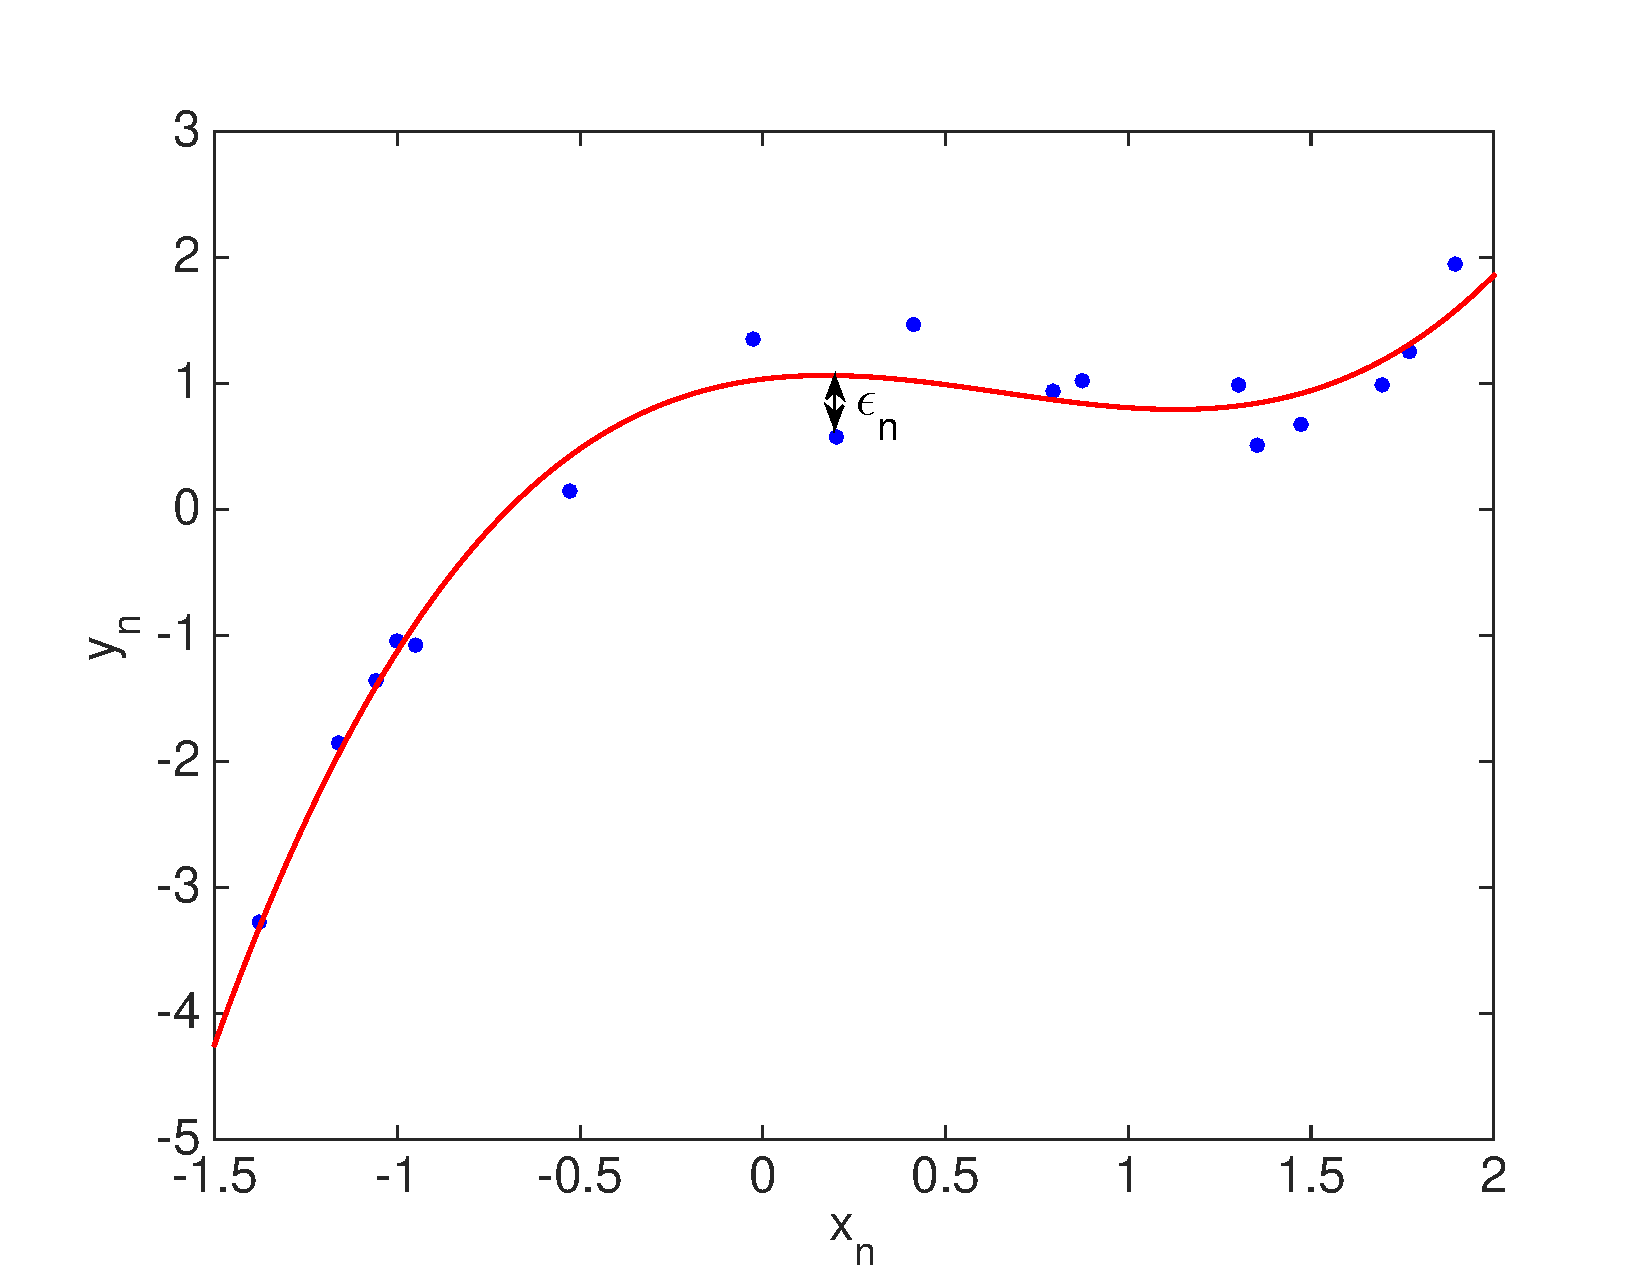
\includegraphics[width=0.5\textwidth]{toy_data_illustrate_Gaussian_noise.pdf}}
\vskip -4mm
\begin{itemize}
\item Imagine the data was in reality \Red{generated} by the \Red{red function}.
\item But each $f(x_*)$ was independently contaminated by a noise term $\epsilon_n$.
\item The observations are noisy: $y_n=f_\bfw(x_n)+\epsilon_n$.
\item We can characterise the noise with a probability density function.\\ 
For example a Gaussian density function, $\epsilon_n\sim\N(\epsilon_n
; \;0, \sigma_\mathrm{noise}^2)$:
\[
p(\epsilon_n)\;=\;\frac{1}{\sqrt{2\pi\,\sigma_\mathrm{noise}^2}}
\exp{\Big(-\frac{\epsilon_n^2}{2\,\sigma_\mathrm{noise}^2}\Big)}
\]
%
\end{itemize}


\end{frame}
%%%%%%%%%%%%%%%%%%%%%%%%%%%%%%%%%%%%%%%%%%%%%%%%%%%%%%%%%%%%%%%%%%%%%%
\begin{frame}
\frametitle{Probability of the observed data given the model}

A vector and matrix notation view of the noise.
\begin{itemize}
\item $\bepsilon=[\epsilon_1,\ldots,\epsilon_N]^\top$ stacks the \Blue{independent} noise terms:
%
\[
\bepsilon\sim\N(\bepsilon;\;\mathbf{0},\,\sigma_\mathrm{noise}^2\bfI)
\hspace{4ex}
p(\bepsilon)=\Blue{\prod_{n=1}^N p(\epsilon_n)}=
\Big(\frac{1}{\sqrt{2\pi\,\sigma_\mathrm{noise}^2}}\Big)^N
\exp{\big(-\frac{\bepsilon^\top\bepsilon}{2\,\sigma_\mathrm{noise}^2}\big)}
\]
% 
\item Given that $\bfy=\bff+\bepsilon$ we can write the probability of $\bfy$ given $\bff$:
%
\begin{align*}
p(\bfy|\bff,\,\sigma_\mathrm{noise}^2)=\N(\bfy;\;\bff,\,\sigma_\mathrm{noise}^2)
&=\Big(\frac{1}{\sqrt{2\pi\,\sigma_\mathrm{noise}^2}}\Big)^N
\exp{\big(-\frac{\|\bfy-\bff\|^2}{2\,\sigma_\mathrm{noise}^2}\big)}\\
&=\Big(\frac{1}{\sqrt{2\pi\,\sigma_\mathrm{noise}^2}}\Big)^N
\exp{\big(-\frac{\Red{E(\bfw)}}{2\,\sigma_\mathrm{noise}^2}\big)}
\end{align*}
%
\item
  $\Red{E(\bfw)}\!=\!\sum_{n=1}^N(y_n-f_\bfw(x_n))^2\!=\!\|\bfy-\bPhi\,\bfw\|^2
  \!= \!\bepsilon^\top\!\bepsilon$ is the sum of squared 
errors
\item Since $\bff=\bPhi\,\bfw$ we can write 
$p(\bfy|\bfw,\,\sigma_\mathrm{noise}^2)=p(\bfy|\bff,\,\sigma_\mathrm{noise}^2)$ for a given $\bPhi$.
\end{itemize}
\end{frame}


\begin{frame}
\frametitle{Likelihood function}

The \Blue{\em likelihood} of the parameters is the probability of the data given
 parameters.
\begin{itemize}
\item $p(\bfy|\bfw,\,\sigma_\mathrm{noise}^2)$ is the probability of the observed data given the 
weights.
\item $\mathcal{L}(\bfw)\propto p(\bfy|\bfw,\,\sigma_\mathrm{noise}^2)$ is the 
likelihood of the weights.
\end{itemize}

\vfill

\Blue{\em Maximum likelihood:}
\begin{itemize}
\item We can fit the model weights to the data by maximising the likelihood:
%
\[
\hat\bfw\;=\;\argmax\; \mathcal{L}(\bfw)
\;=\;\argmax\;\exp{\big(-\frac{E(\bfw)}{2\,\sigma_\mathrm{noise}^2}\big)}
\;=\;\argmin\; E(\bfw)
\]
%
\item With an additive Gaussian independent noise model, the \Red{maximum likelihood} and the 
\Red{least squares} solutions are the same.
\item But... we still have not solved the prediction problem! We still overfit.

\end{itemize}

\end{frame}
%%%%%%%%%%%%%%%%%%%%%%%%%%%%%%%%%%%%%%%%%%%%%%%%%%%%%%%%%%%%%%%%%%%%%%
\begin{frame}
\frametitle{Multiple explanations of the data}

\vspace{-0.5ex}
\begin{itemize}
\item We do not \Blue{believe} all models are equally probable to explain the data.
\item We may \Blue{believe} a simpler model is more probable than a complex one.
\end{itemize}
%
Model complexity and uncertainty:
\vspace{-0.5ex}
\begin{itemize}
\item We do not \Blue{know} what particular function generated the data.
\item More than one of our models can perfectly fit the data.
\item We \Blue{believe} more than one of our models could have generated the data.
\item We want to reason in terms of \Red{a set of possible explanations}, not just one.
\end{itemize}
%
\centerline{
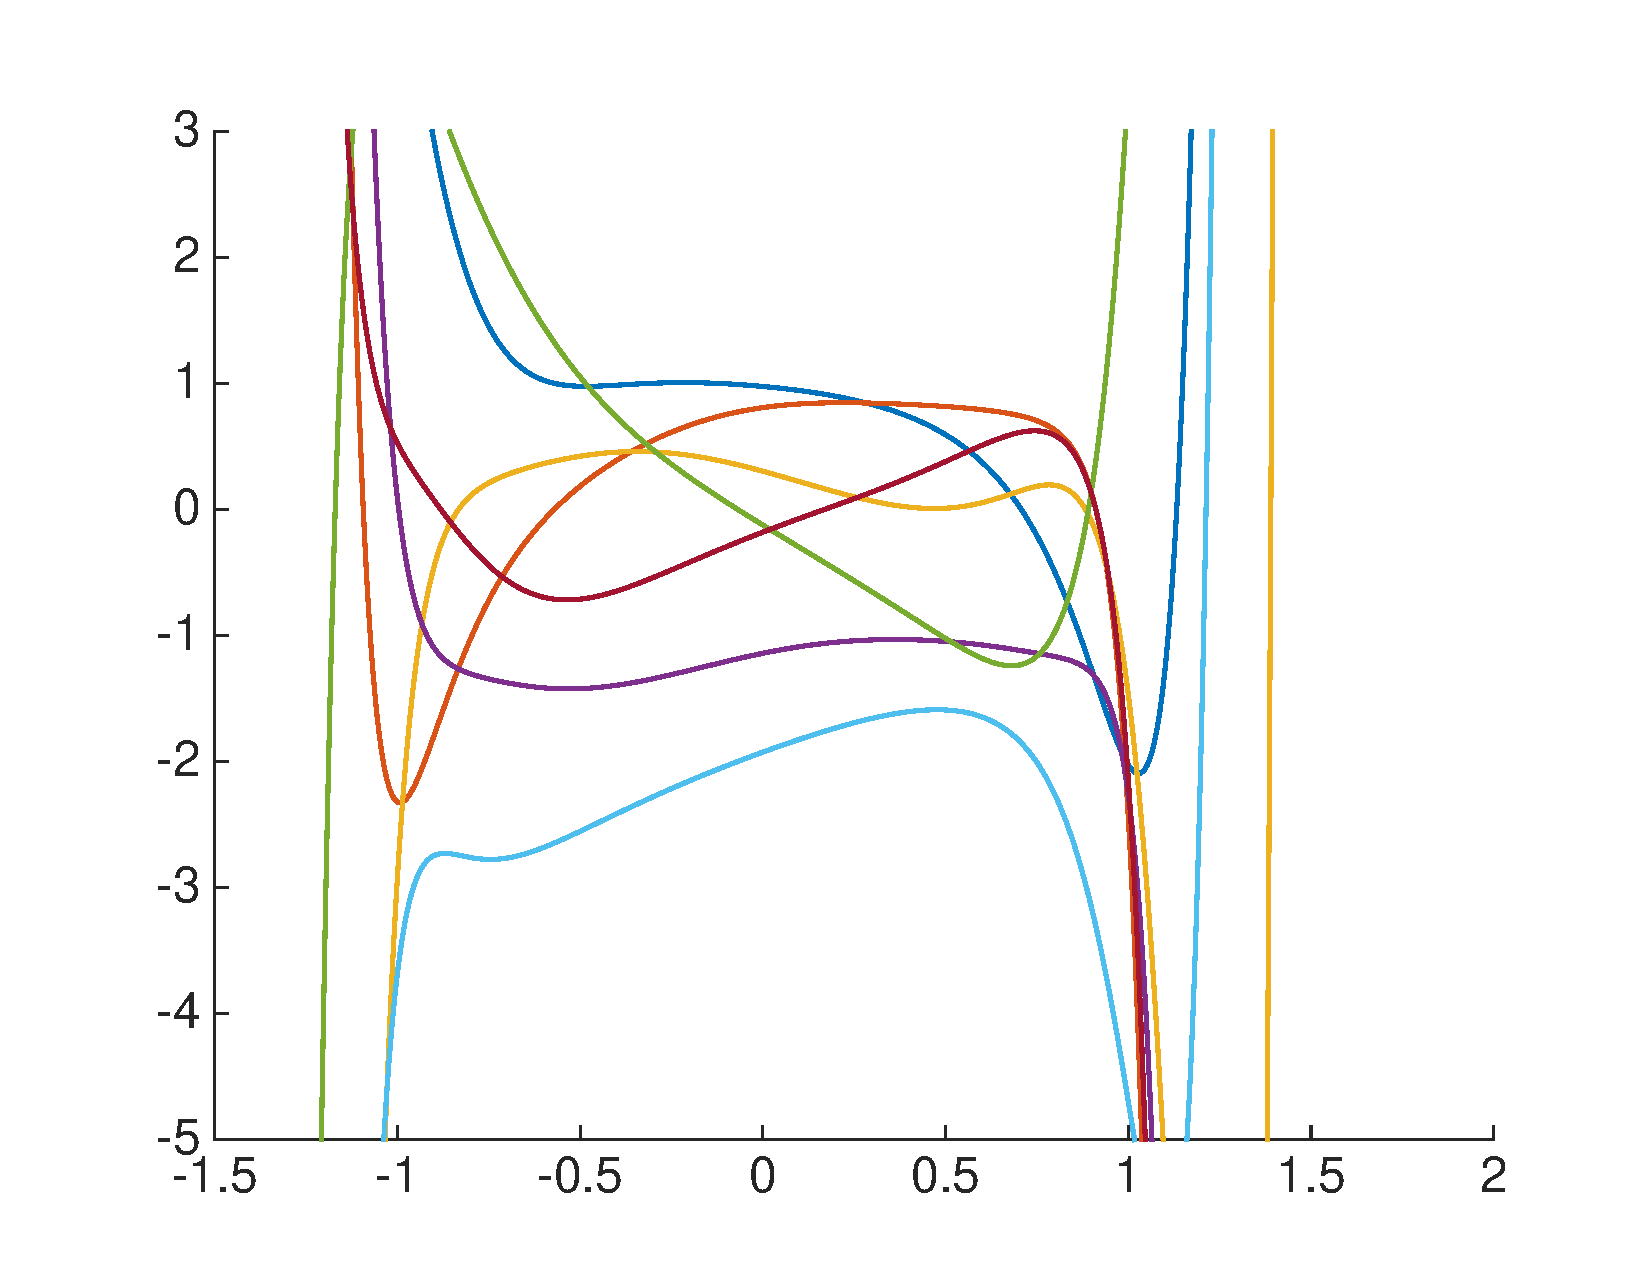
\includegraphics[width=0.45\textwidth]{random_polynomials_degree17.pdf}
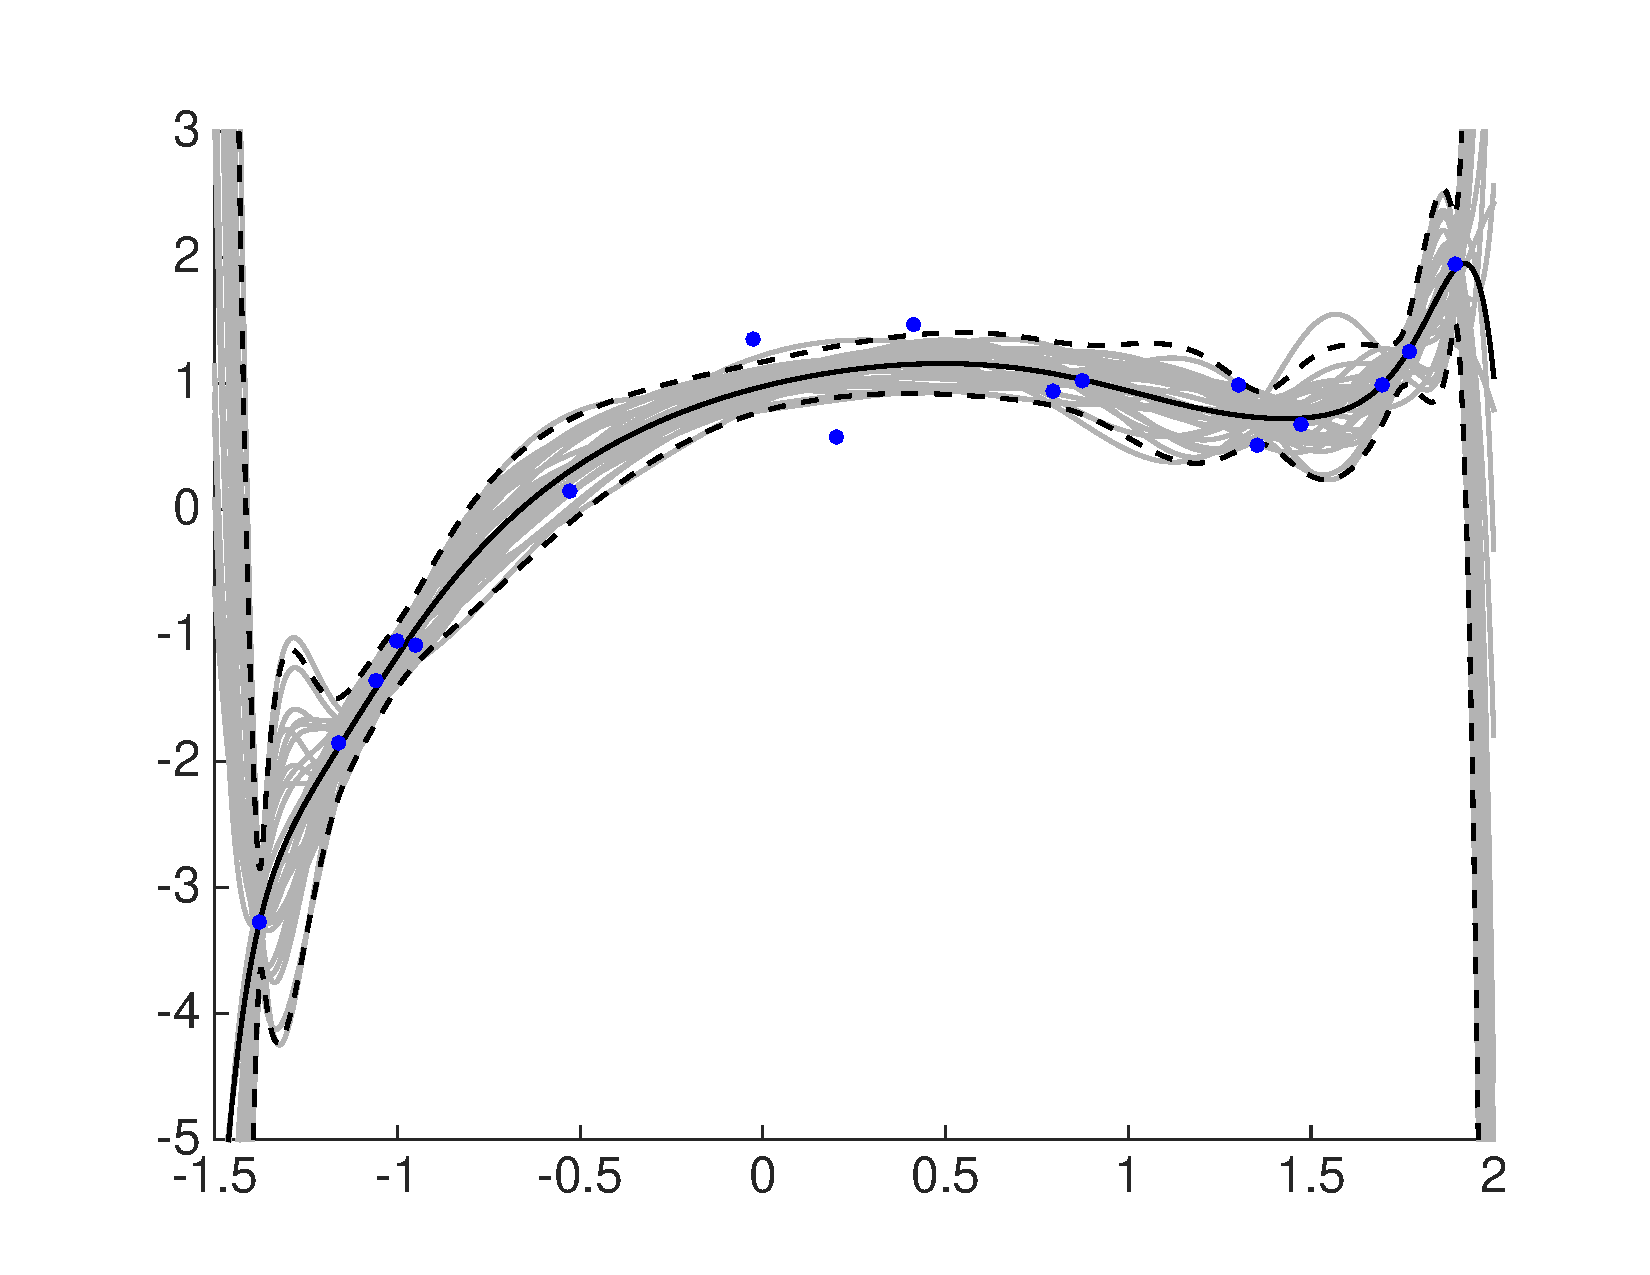
\includegraphics[width=0.45\textwidth]{samples_posterior_degree17.pdf}
}
%

\end{frame}
\end{document}
